% This file was created with tikzplotlib v0.9.15.
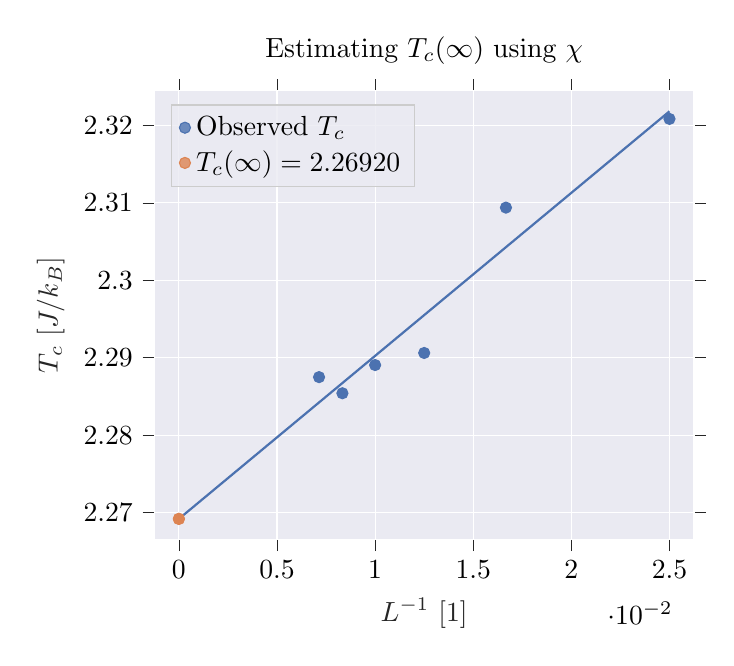
\begin{tikzpicture}

\definecolor{color0}{rgb}{0.917647058823529,0.917647058823529,0.949019607843137}
\definecolor{color1}{rgb}{0.298039215686275,0.447058823529412,0.690196078431373}
\definecolor{color2}{rgb}{0.866666666666667,0.517647058823529,0.32156862745098}

\begin{axis}[
axis background/.style={fill=color0},
axis line style={white},
legend cell align={left},
legend style={
  fill opacity=0.8,
  draw opacity=1,
  text opacity=1,
  at={(0.03,0.97)},
  anchor=north west,
  draw=white!80!black,
  fill=color0
},
tick align=outside,
title={Estimating \(\displaystyle T_c(\infty)\) using \(\displaystyle \chi\)},
x grid style={white},
xlabel=\textcolor{white!15!black}{\(\displaystyle L^{-1}\) [1]},
xmajorgrids,
xmajorticks=true,
xmin=-0.00125, xmax=0.02625,
xtick style={color=white!15!black},
y grid style={white},
ylabel=\textcolor{white!15!black}{\(\displaystyle T_c\) [\(\displaystyle J / k_B\)]},
ymajorgrids,
ymajorticks=true,
ymin=2.26657395139442, ymax=2.32443954342629,
ytick style={color=white!15!black}
]
\addplot [draw=color1, fill=color1, mark=*, only marks]
table{%
x  y
0.0249999999999999 2.32083
0.0166666666666666 2.30938
0.0125 2.29062
0.01 2.28906
0.0083333333333333 2.28542
0.00714285714285712 2.2875
};
\addlegendentry{Observed $T_c$}
\addplot [draw=color2, fill=color2, mark=*, only marks]
table{%
x  y
0 2.26920420557769
0 2.26920420557769
};
\addlegendentry{$T_c(\infty) =  2.26920$}
\addplot [thick, color1, forget plot]
table {%
0 2.26920413970947
0.0249999761581421 2.3218092918396
};
\end{axis}

\end{tikzpicture}
